% The Turan graph T(10,3) (generated by figs_c1ch08.py).
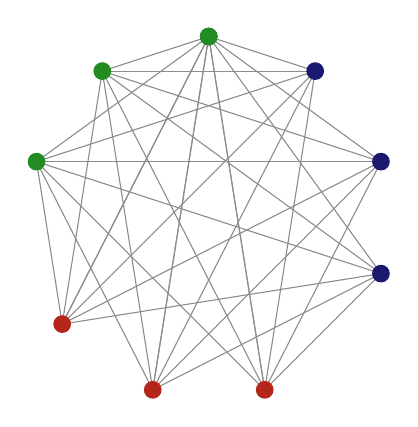
\begin{tikzpicture}[x=1cm,y=1cm,v/.style={circle,fill=MidnightBlue,inner sep=1.6pt},e/.style={MidnightBlue!70},l/.style={font=\footnotesize}]
\draw[black!45] (0.000,2.300) -- (0.711,-2.187);
\draw[black!45] (0.000,2.300) -- (-0.711,-2.187);
\draw[black!45] (0.000,2.300) -- (-1.861,-1.352);
\draw[black!45] (0.000,2.300) -- (-2.187,0.711);
\draw[black!45] (0.000,2.300) -- (-1.352,1.861);
\draw[black!45] (0.000,2.300) -- (-0.000,2.300);
\draw[black!45] (1.352,1.861) -- (0.711,-2.187);
\draw[black!45] (1.352,1.861) -- (-0.711,-2.187);
\draw[black!45] (1.352,1.861) -- (-1.861,-1.352);
\draw[black!45] (1.352,1.861) -- (-2.187,0.711);
\draw[black!45] (1.352,1.861) -- (-1.352,1.861);
\draw[black!45] (1.352,1.861) -- (-0.000,2.300);
\draw[black!45] (2.187,0.711) -- (0.711,-2.187);
\draw[black!45] (2.187,0.711) -- (-0.711,-2.187);
\draw[black!45] (2.187,0.711) -- (-1.861,-1.352);
\draw[black!45] (2.187,0.711) -- (-2.187,0.711);
\draw[black!45] (2.187,0.711) -- (-1.352,1.861);
\draw[black!45] (2.187,0.711) -- (-0.000,2.300);
\draw[black!45] (2.187,-0.711) -- (0.711,-2.187);
\draw[black!45] (2.187,-0.711) -- (-0.711,-2.187);
\draw[black!45] (2.187,-0.711) -- (-1.861,-1.352);
\draw[black!45] (2.187,-0.711) -- (-2.187,0.711);
\draw[black!45] (2.187,-0.711) -- (-1.352,1.861);
\draw[black!45] (2.187,-0.711) -- (-0.000,2.300);
\draw[black!45] (0.711,-2.187) -- (-2.187,0.711);
\draw[black!45] (0.711,-2.187) -- (-1.352,1.861);
\draw[black!45] (0.711,-2.187) -- (-0.000,2.300);
\draw[black!45] (-0.711,-2.187) -- (-2.187,0.711);
\draw[black!45] (-0.711,-2.187) -- (-1.352,1.861);
\draw[black!45] (-0.711,-2.187) -- (-0.000,2.300);
\draw[black!45] (-1.861,-1.352) -- (-2.187,0.711);
\draw[black!45] (-1.861,-1.352) -- (-1.352,1.861);
\draw[black!45] (-1.861,-1.352) -- (-0.000,2.300);
\fill[MidnightBlue] (0.000,2.300) circle (3.2pt);
\fill[MidnightBlue] (1.352,1.861) circle (3.2pt);
\fill[MidnightBlue] (2.187,0.711) circle (3.2pt);
\fill[MidnightBlue] (2.187,-0.711) circle (3.2pt);
\fill[BrickRed] (0.711,-2.187) circle (3.2pt);
\fill[BrickRed] (-0.711,-2.187) circle (3.2pt);
\fill[BrickRed] (-1.861,-1.352) circle (3.2pt);
\fill[ForestGreen] (-2.187,0.711) circle (3.2pt);
\fill[ForestGreen] (-1.352,1.861) circle (3.2pt);
\fill[ForestGreen] (-0.000,2.300) circle (3.2pt);
\end{tikzpicture}
